% Hinh: paper/paper1_qmi/figs_revision/fig5 (make_paper1_figures.py --qmi). Caption viet lai cho QMI.
\begin{figure}[t]
  \centering
  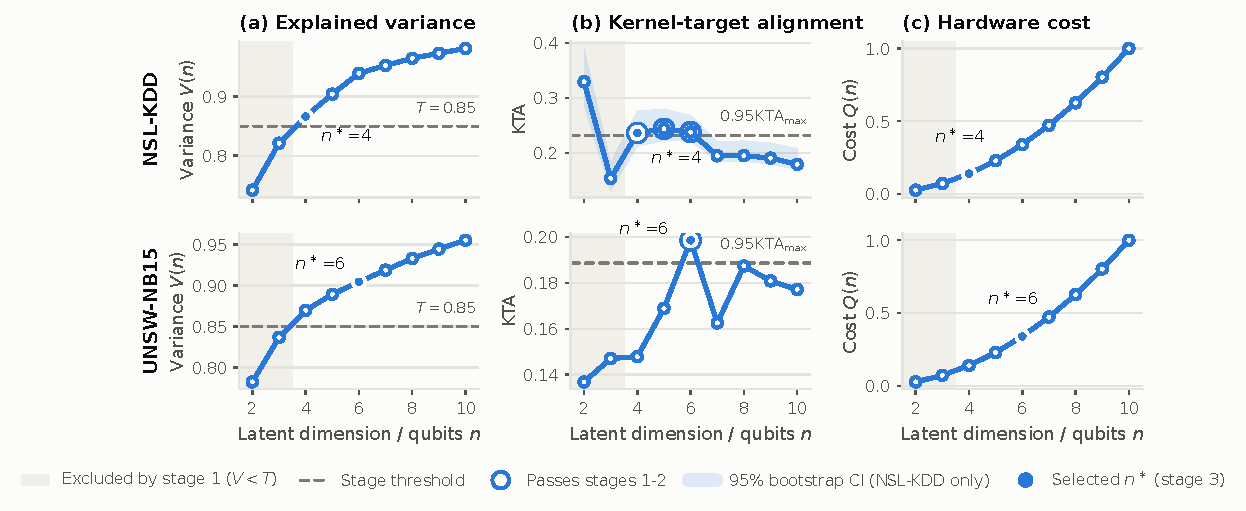
\includegraphics[width=\textwidth]{figs_revision/fig5_c1_dimension_selection.pdf}
  \caption{The three-stage width-selection rule on NSL-KDD (top) and UNSW-NB15 (bottom).
    (a) Cumulative explained variance $V(n)$; (b) kernel--target alignment; (c) CNOT-weighted
    cost $Q(n)$. Stage~1 discards $V(n)<0.85$ (shaded), stage~2 keeps
    $\mathrm{KTA}\ge0.95\,\mathrm{KTA}_{\max}$ (open circles), and stage~3 takes the cheapest
    remaining width (filled). The rule returns $n^{\ast}=4$ and $n^{\ast}=6$ with the same
    thresholds.}
  \label{fig:c1-selection}
\end{figure}
